%%%%%%%%%%%%%%%%%%%%%%%%%%%%%%%%%%%%%%%%%
% baposter Portrait Poster
% LaTeX Template
% Version 1.0 (15/5/13)
%
% Created by:
% Brian Amberg (baposter@brian-amberg.de)
%
% This template has been downloaded from:
% http://www.LaTeXTemplates.com
%
% License:
% CC BY-NC-SA 3.0 (http://creativecommons.org/licenses/by-nc-sa/3.0/)
%
%%%%%%%%%%%%%%%%%%%%%%%%%%%%%%%%%%%%%%%%%

%----------------------------------------------------------------------------------------
%	PACKAGES AND OTHER DOCUMENT CONFIGURATIONS
%----------------------------------------------------------------------------------------

\documentclass[a0paper,portrait]{baposter}

\usepackage[font=small,labelfont=bf]{caption} % Required for specifying captions to tables and figures
\usepackage{booktabs} % Horizontal rules in tables
\usepackage{relsize} % Used for making text smaller in some places
\usepackage{url}

\graphicspath{{figures/}} % Directory in which figures are stored

\definecolor{bordercol}{RGB}{40,40,40} % Border color of content boxes
\definecolor{headercol1}{RGB}{186,215,230} % Background color for the header in the content boxes (left side)
\definecolor{headercol2}{RGB}{80,80,80} % Background color for the header in the content boxes (right side)
\definecolor{headerfontcol}{RGB}{0,0,0} % Text color for the header text in the content boxes
\definecolor{boxcolor}{RGB}{186,215,230} % Background color for the content in the content boxes
\definecolor{contrastcol}{RGB}{250,85,10} % Contrast color
\definecolor{emphsizecol}{RGB}{100,250,100} % Contrast color

\begin{document}

\background{ % Set the background to an image (background.pdf)
\begin{tikzpicture}[remember picture,overlay]
\draw (current page.north west)+(-2em,2em) node[anchor=north west]
{\includegraphics[height=1.1\textheight]{background}};
\end{tikzpicture}
}

\begin{poster}{
grid=false,
borderColor=bordercol, % Border color of content boxes
headerColorOne=headercol1, % Background color for the header in the content boxes (left side)
headerColorTwo=headercol2, % Background color for the header in the content boxes (right side)
headerFontColor=headerfontcol, % Text color for the header text in the content boxes
boxColorOne=boxcolor, % Background color for the content in the content boxes
headershape=roundedright, % Specify the rounded corner in the content box headers
headerfont=\Large\sf\bf, % Font modifiers for the text in the content box headers
textborder=rectangle,
background=user,
headerborder=open, % Change to closed for a line under the content box headers
boxshade=plain
}
{}
%
%----------------------------------------------------------------------------------------
%	TITLE AND AUTHOR NAME
%----------------------------------------------------------------------------------------
%
{\sf\bf \LARGE{Sammba-MRI: SmAll MaMmals BrAin MRI in Python}} % Poster title
{\vspace{1em} Salma Bougacha{\textsuperscript{1,2}}, Nachiket Nadkarni\textsuperscript{1}, Cl\'ement Garin\textsuperscript{1}, Marc Dhenain\textsuperscript{1}\\ % Author names
{\small 1  Neurodegenerative Dis. Lab., MIRCen, CEA, Fontenay aux Roses Cedex, France;
2  U1077, INSERM, Caen, France}} % Author email addresses
{
\includegraphics[scale=0.4]{cyceron_mircen.png}} % University/lab logo

%----------------------------------------------------------------------------------------
%	INTRODUCTION
%----------------------------------------------------------------------------------------

\headerbox{Introduction}{name=introduction,column=0,row=0}{

The available software for \textcolor{emphsizecol}{\textbf{processing Small mammals neuroimaging}} data lacks maturity:

\begin{itemize}
\item Bruker DICOM to NIFTI conversion is not guaranteed
\item Manual intervention is usually needed
\item Can perform badly or even fail depending on the images quality
\end{itemize}

sammba-MRI
enables fluent scriptable analysis workflows, from DICOM conversion to results visualization.

}

%----------------------------------------------------------------------------------------
%	DATA
%----------------------------------------------------------------------------------------

\headerbox{Data}{name=data,column=0,below=introduction}{

\begin{center}
\begin{tabular}{l l l}
\toprule
\textbf{Dataset} & \textbf{Animals} & \textbf{scans} \\
\midrule
Brookhave 			& 12 C57 mice 		& anat T2 			  \\ %BL/6J, Bruker 9.4 T
2008 \cite{ma:2008} & 3-4 months 		&					 	    \\%12-14 weeks
	 	  			&					&							\\
Inhouse 	  & 34 lemurs 		& anat T2 			\\% Bruker 11.7 T
2017 	  &	15-60 months  	&							\\
	 	  &					&							\\
Inhouse	  &	10 C57 mice 		& anat T2  			\\% Bruker 11.7 T
2017	  	  & 5-7 months 		& perfusion			  		\\
	 	  &					&							\\
Zerbi 	  & 15 C57 mice 		& anat T2 			 \\% Bruker 9.4 T
2015 \cite{zerbi:2015} 	  & 2-3 months  	& BOLD-EPI   		 		\\
\bottomrule
\end{tabular}
\captionof{table}{Data characteristics}
\end{center}
 
}

%----------------------------------------------------------------------------------------
%	MATERIAL AND METHODS
%----------------------------------------------------------------------------------------

\headerbox{Materials and Methods}{name=methods,column=0,below=data}{

Fusce at erat vitae metus porttitor auctor sit amet at ante. In id dolor tellus, non aliquet elit. Vestibulum bibendum, augue sed laoreet congue, enim nisi ultricies diam, ac pharetra mi dui ut sapien. Maecenas fermentum, neque ut scelerisque consequat, purus leo ultrices nulla, quis scelerisque risus elit non turpis. 

\begin{enumerate}
\item Cras ac ipsum eu nisl imperdiet interdum nunc bibendum, est in pulvinar facilisis, mi purus fringilla tellus, eu varius ipsum ante laoreet ipsum
\item Sed cursus erat quis odio laoreet facilisis maecenas vehicula
\end{enumerate}
}

%----------------------------------------------------------------------------------------
%	REFERENCES
%----------------------------------------------------------------------------------------

\headerbox{References}{name=references,column=0,below=methods, above=bottom}{

\smaller % Reduce the font size in this block
\renewcommand{\section}[2]{\vskip 0.05em} % Get rid of the default "References" section title
\nocite{*} % Insert publications even if they are not cited in the poster

\bibliographystyle{unsrt}
\bibliography{sample} % Use sample.bib as the bibliography file
}

%----------------------------------------------------------------------------------------
%	RESULTS 1
%----------------------------------------------------------------------------------------

\headerbox{Results 1: Registration accuracy}{name=results1,span=2,column=1,row=0}{ % To reduce this block to 1 column width, remove 'span=2'

Nunc sit amet sem ut nulla tincidunt mattis vel nec mauris. Vestibulum odio tellus, lobortis. Vel adipiscing, Aliquam dictum, ligula egestas commodo posuere, lectus lectus congue ligula, sed posuere urna lectus at nisi. Aenean commodo risus ut dolor (viverra scelerisque). Nullam varius, lacus et interdum hendrerit, odio orci ultrices mauris, id interdum eros mauris at urna. Fusce in nisi eros, sit amet volutpat turpis, \textbf{porttior magna} (commodo blandit euismod) \textbf{facilisis ornate magnis} (dis magnis). 

%------------------------------------------------

\begin{center}
\begin{tabular}{l l l}
\toprule
\textbf{Treatments} & \textbf{Response 1} & \textbf{Response 2}\\
\midrule
Treatment 1 & 0.0003262 & 0.562 \\
Treatment 2 & 0.0015681 & 0.910 \\
Treatment 3 & 0.0009271 & 0.296 \\
\bottomrule
\end{tabular}
\captionof{table}{Table caption}
\end{center}
}

%----------------------------------------------------------------------------------------
%	RESULTS 2
%----------------------------------------------------------------------------------------

\headerbox{Results 2: Group studies}{name=results2,span=2,column=1,below=results1,above=bottom}{ % To reduce this block to 1 column width, remove 'span=2'
\textbf{\large{\textcolor{contrastcol}{Template creation}}}
Studying   populations   of   animals   gains   precision   by   the   use   of   cohort   specific   templates.  
Sammba-MRI   proposes   an   iterative   method   to   create   a   fine   anatomical   template   from   individual  
structural   MRI   scans.   We   show   in   Figure \ref{fig:template}   the template  created   from   34   mouse  
lemurs (inhouse dataset). The method adapts to different animal species.

\begin{center}
\label{fig:template}
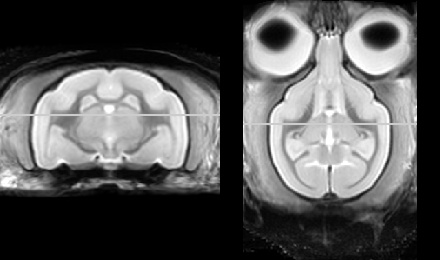
\includegraphics[width=0.4\linewidth]{sfn_template.jpg}
\captionof{figure}{mouse lemur template}
\end{center}
%------------------------------------------------
\textbf{\large{\textcolor{contrastcol}{Cerebral Blood Flow quantification}}}
Estimating   the   cerebral   blood   flow   (CBF)   in   animals   is   challenging   due   to   the   low   SNR   and   lack   of  
sensitivity.   Sammba-MRI   allows   to   estimate   quantitative   CBF   maps   for   Bruker-FAIR   EPI  
sequences. Figure 2 shows CBF map from a group of 10 mice (inhouse dataset). 

%------------------------------------------------
\begin{center}
\label{fig:cbf}
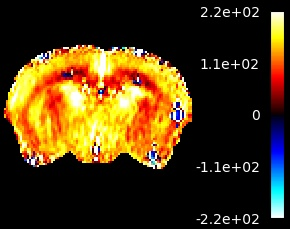
\includegraphics[width=0.4\linewidth]{mean_cbf_y_no_title.jpg}
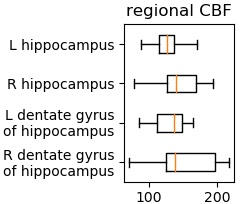
\includegraphics[width=0.4\linewidth]{regional_cbf_4rois.jpeg}
\captionof{figure}{Group   average   CBF   map (left); individual regional CBF in ml/100g/min (right)}
\end{center}

%------------------------------------------------
\textbf{\large\textcolor{contrastcol}{{Resting state networks}}}
Resting   state   spatial   networks   extraction   can   be   done   using   ICA.   Using   sammba-MRI,   we  
performed   ICA   on   a   group   of   15   mice      from   a   public   dataset   [6].   Relevant   bilateral  
regions are found even ​ without data post-processing ​ (Figures 3 and 4).

%------------------------------------------------
\begin{center}
\includegraphics[width=0.17\linewidth]{{component1.jpg}}
\includegraphics[width=0.17\linewidth]{{component5.jpg}}
\includegraphics[width=0.17\linewidth]{{component9.jpg}}
\includegraphics[width=0.17\linewidth]{{component10.jpg}}
\includegraphics[width=0.17\linewidth]{{component13.jpg}}
\includegraphics[width=0.17\linewidth]{{component16.jpg}}
\includegraphics[width=0.17\linewidth]{{component17.jpg}}
\includegraphics[width=0.17\linewidth]{{component21.jpg}}
\includegraphics[width=0.17\linewidth]{{component26.jpg}}
\captionof{figure}{Bilateral ICA components}
\end{center}

%------------------------------------------------

\begin{center}
\large{\textcolor{emphsizecol}{\url{https://sammba-mri.github.io/}}}
\end{center}
}
%----------------------------------------------------------------------------------------

\end{poster}

\end{document}